\documentclass[11pt,twoside]{article}
\usepackage[T1]{fontenc}
\usepackage[english]{babel}
\usepackage[utf8]{inputenc}

\usepackage{amsmath}
\usepackage{amscd}
\usepackage{amssymb}
\usepackage{tabularx}
\usepackage{url}
\usepackage{fancyhdr}
\usepackage[a4paper,margin=2.5cm,hmarginratio=1:1]{geometry}
\usepackage{graphicx}
\usepackage{pdfpages}

\title{Kometens Stoftsvans}
\author{Joakim Uddholm, juddholm@kth.se, 9110013290 \\
		Jo Tryti, tryti@kth.se, 8612050438}
\date{}

\begin{document}
\maketitle
\newpage
\includepdf[pages=22]{Lab3BuppgJO.pdf}

\section{Kometens bana}

\subsection{Kometens radie}
Radien för en komets eliptiska bana fås av:
\begin{equation}
    r(\phi)=\frac{R}{1-E\cos\phi}
\end{equation}
I vår fall undersöker vi den specifika banan som fås utav:
\begin{equation}
	\begin{split}
     R = 105, E = 0.4, 0 \leq \phi \leq 2\pi \\
     r(\phi)=\frac{105}{1-0.4\cos\phi}
     \end{split}
\end{equation}
Med derivatan som vi senare kommer använda för kometens riktning
\begin{equation}
    r'(\phi)=\frac{42}{(1-0.4\cos\phi)^2}
\end{equation}

\section{Kometens riktning}	
Med radien $r(\phi)$ fås en positionsvektor $P(\phi)$.
\begin{equation}
	P(\phi) = \begin{cases}
	x = r(\phi) cos(\phi) \\
	y = r(\phi) sin(\phi)
	\end{cases}
\end{equation}
Den partiella derivatan av ovanstående funktion ger riktningen $k$ som en funktion av $\phi$. 
\begin{equation}
	k(\phi) = \begin{cases}
	x = r'(\phi) cos(\phi) - r(\phi) sin(\phi) \\
	y = r'(\phi) sin(\phi) + r(\phi) cos(\phi)
	\end{cases}
\end{equation}

\section{Randvärdet kometens hastighet}



\section{Stoftpartiklarna}



\end{document}
